\section{Convergence}
\label{AppendixD}
\subsection*{General Aim}
When conducting a FEM simulation, convergence must be considered. Convergence is the act of the Nodal and the elemental stress converging to a single value. During the solution process, in each element, stress results are calculated at certain locations called Gauss points. Nodal Stresses in Gauss points can be extrapolated to element nodes. Most often, one node is shared by several elements, and each element reports different stresses at the shared node. Reported values from all adjacent elements are then averaged to obtain a single value. This method of stress averaging produces nodal stress results. 

Elemental values Alternately, the stress values from all Gaussian points within each element can be averaged to report a single elemental stress. Although these stresses are averaged between Gauss points, they are called non-averaged 
stresses (or elemental stresses) because the averaging is done internally within the same element only.

As the amount of gauss points goes to infinity the nodal and elemental stress will reach the same value. As it is impossible to create an infinite amount of measurement points, a method to determine a mesh size where the stresses remain the same even as the mesh is refined must be determined. 

\subsection*{Convergence Study}
The convergence study was completed to determine an adequate difference between both mesh refinements and elemental and nodal stresses. As is explained above, mesh refinements will have less of an effect on the stresses as the stresses begin to converge. In addition to this, the differences between elemental and nodal will also decrease as the stresses converge. The differences in elemental and nodal stresses will show whether the solution is converging. The changes between mesh refinements will give an indication of where convergence occurs; this is particularly important for the convergence definition of the stator. If the mesh refinements have little affect at a point with a small difference between elemental and nodal stresses, the convergence percentage can be determined at that point.
\begin{equation}
convergence\quad \%  = \frac{\sigma_{elemental-nodal} - \sigma_{elemental} }{\sigma_{elemental-nodal}} \cdot 100
\end{equation}
Convergence percentage will be particularly useful for the validation of any FEM simulation results as it determines whether the stresses have converged, independent of particular mesh sizes. This is logical, as different areas require different mesh refinement techniques \cite{convergence}.
\subsection*{Convergence of the Stator}
To determine the convergence percentage in the stator, a 3D mesh type CTETRA(10) is used. In order to complete the convergence study on the stator, stress measurement points had to be determined. As the critical points for the analysis occur near the edges of the blade of the stator, the area around the edge is analyzed in terms of elemental and nodal stresses for various mesh sizes. A 3D partitioned model is used at the high stress areas to simulate realistic results in the top of the stator as well as for the bottom. For the top part the 3D partitioned part can be seen in Figure \ref{partitiontop}.

\begin{figure}[H]
\centering
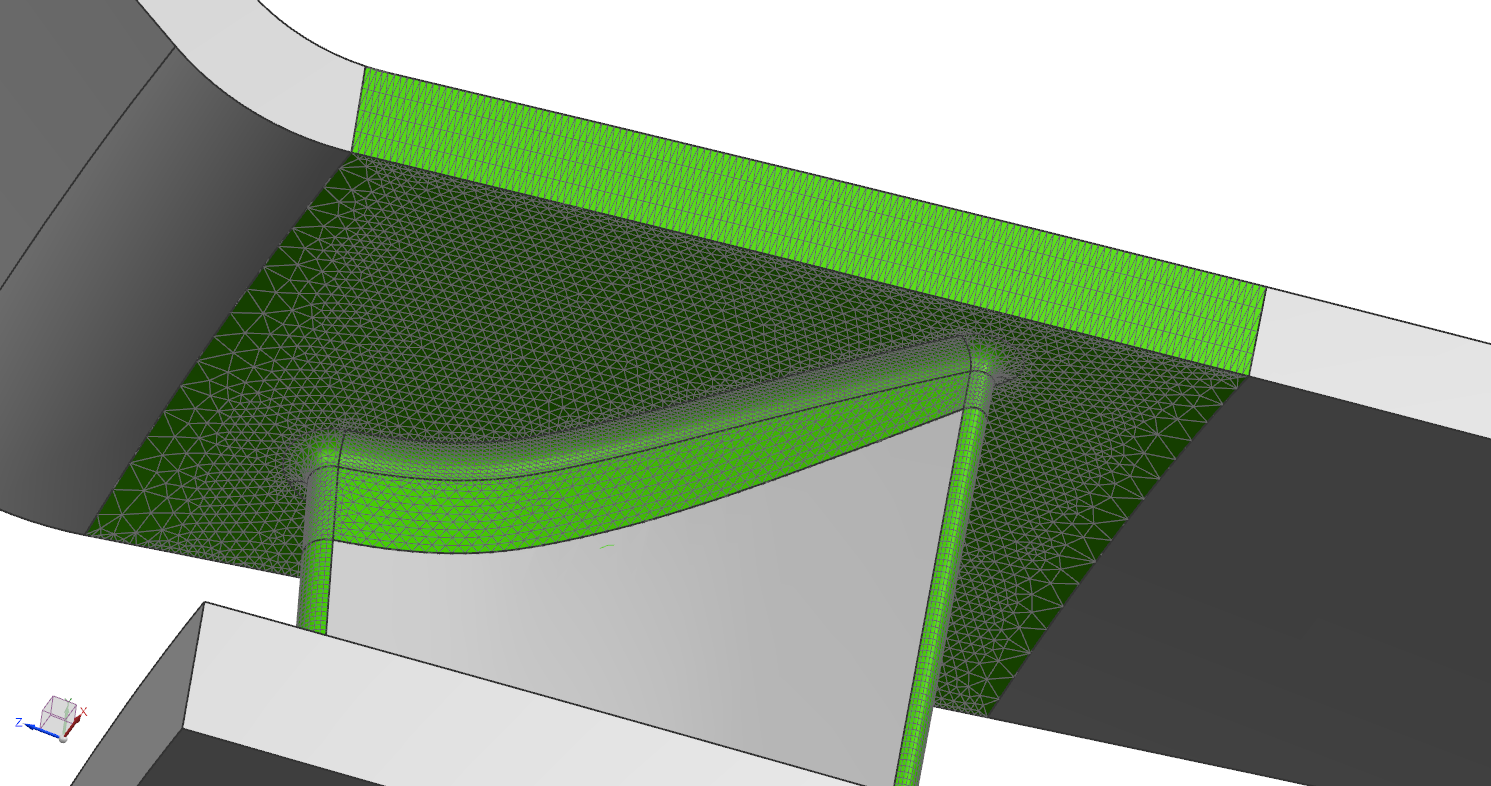
\includegraphics[width=12cm]{Figures/partition_part.png}
\caption{The high stress area during shut-down of the original stator}
\label{partitiontop}
\end{figure}

The convergence is shown in Figure \ref{fig:stress_convergence}. The maximum principal stress of both nodal and elemental are displayed as well.
\begin{figure}[H]
\centering
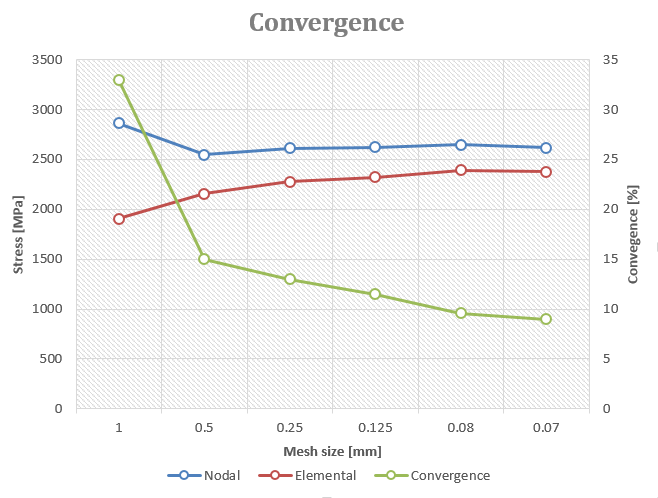
\includegraphics[width=14cm]{Figures/partition.png}
\caption{Convergence analysis for an area near the edge of the blade}
\label{fig:stress_convergence}
\end{figure}
The convergence analysis resulted in a general convergence percentage of 10\%. Certain areas of the stator achieved much lower convergence percentages with refinement; however, the areas near the blade did not seem to converge much further than 10\%. This percentage will be used throughout the stator validation as it can be applied for much more of the stator than a lower percentage which is only achieved at areas with lower stresses.